\documentclass{article}
\usepackage{hyperref}
\usepackage{enumitem}
\usepackage[margin=1in]{geometry}
\usepackage{graphicx}
\usepackage{fancyhdr}
\usepackage{minted}
\usepackage{float}
\graphicspath{{Images/}}

\hypersetup{
	colorlinks=true, %set true if you want colored links
	linkcolor=black,  %choose some color if you want links to stand out
}

\pagestyle{fancy}
\rfoot{
\includegraphics[scale=0.4]{IITlogo}}

\title{ECE 100 Laboratory 02 Instructions }
\author{Illinois Institute of Technology ECE Department}
\date{Last Modified: \today}



\begin{document}
	\maketitle
	
	\paragraph{Lab Objective}
	Build a line follower robot to compete in Competition 1. The most optimal robot will complete the course in its entirety in the shortest amount of time.
	
	\paragraph{Extra Credit} Use the remote control to stop the robot once it passes the finish line.
	
	\section{Hardware Installation}
	
	\paragraph{} Below are the instructions on how to properly assemble the line follower robot. Please follow the instructions as listed to complete the build by the end of the Lab section. The instructions provided below are adapted from the OSOYOO provided instructions for your ease of use. If you wish to have additional support in the build process, navigate to the following link for a video tutorial. 
	
	\href{https://osoyoo.com/2020/05/12/osoyoo-v2-1-robot-car-kit-lesson-4-tracking-line-robot-car/}{Video Tutorial Link}
	
	\begin{enumerate}
		\item Start the installation from the previous status of lab 1.
		
		\item Install tracking sensor modules under lower car chassis with 2pcs M3 plastic screws, M3 plastic pillars, and M3 plastic nuts.
		
		\begin{figure}[H]
			\centering
			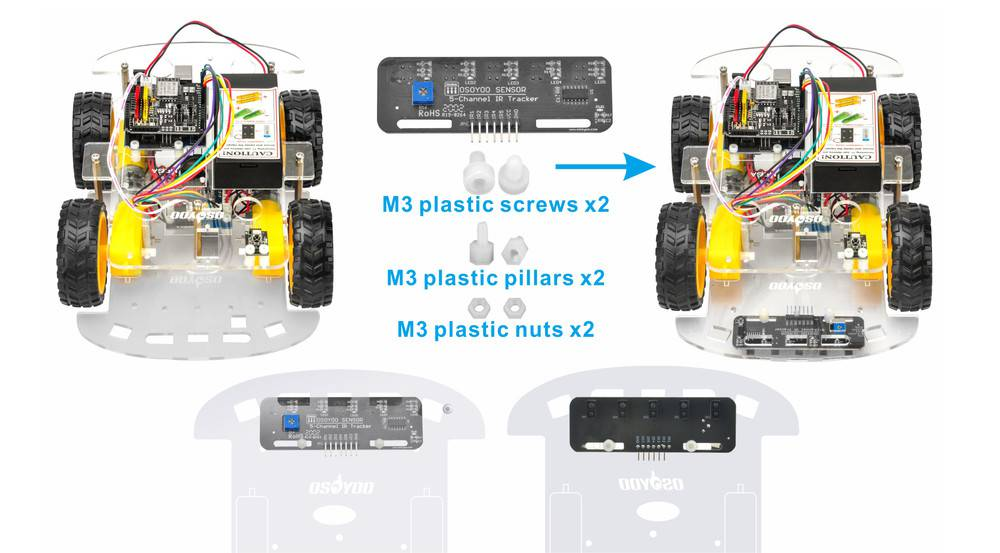
\includegraphics[width=0.7\linewidth]{image2}
			\label{fig:image2}
		\end{figure}
		
		\item Connect the GND-VCC pin of the tracking sensor module to the GND-5V of OSOYOO Uart WiFi shield V1.3.  Connect IR1, IR2, IR3, IR4, IR5 pins to A0, A1, A2, A3, A4 with a 7pin 25cm female to female cable (Remember: DO NOT remove any existing wires installed in Lesson 1 ).
		
		\begin{figure}[H]
			\centering
			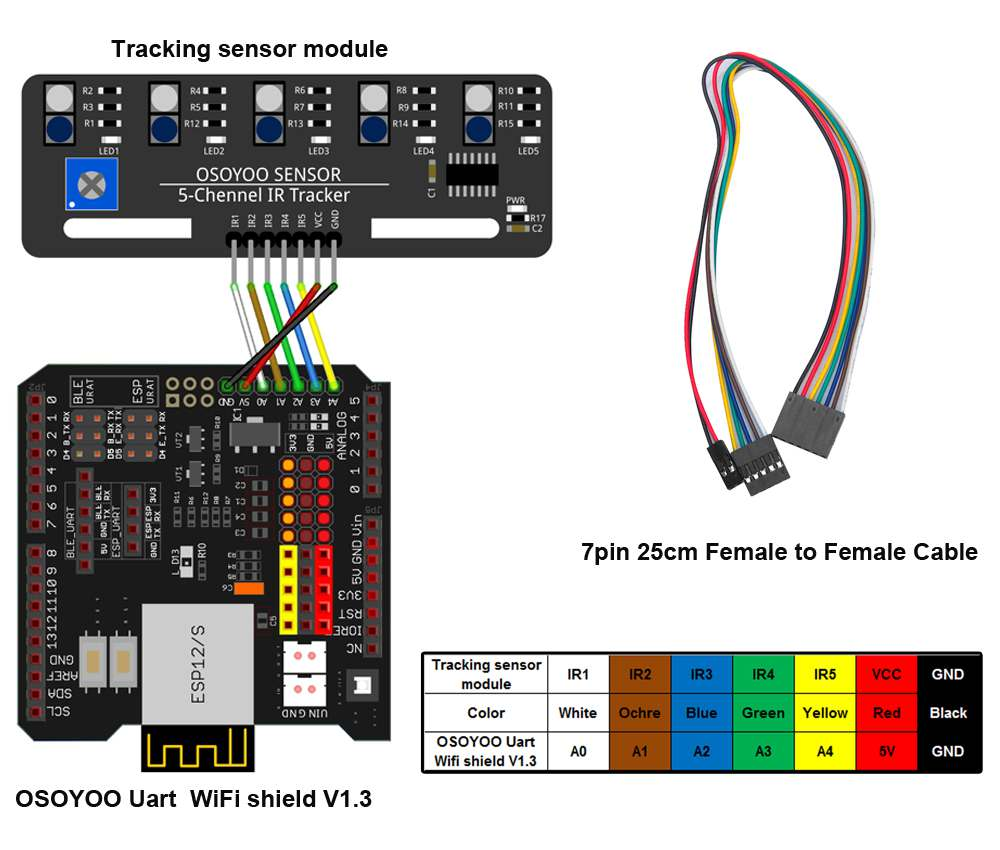
\includegraphics[width=0.7\linewidth]{image3}
			\label{fig:image3}
		\end{figure}
		
	\end{enumerate}

\paragraph{} \textbf{Note: The cable colors might not be identical to the ones in the diagram but make sure that they are properly connected.}

\section{Software Installation}


\begin{enumerate}
	\item Download Lesson 4 tracking smart car sample code from \href{example.com}{v2smartcar-lesson4}. Unzip the download zip file smartcar-lesson4.zip, you will see a folder called smartcar-lesson4B.
	
	\item Connect UNO R3 board to PC with USB cable, Open Arduino IDE $\rightarrow$ click file $\rightarrow$ click Open $\rightarrow$ choose code “smartcar-lesson4.ino” in smartcar-lesson4 folder, load the code into arduino.
	
	\begin{figure}[H]
		\centering
		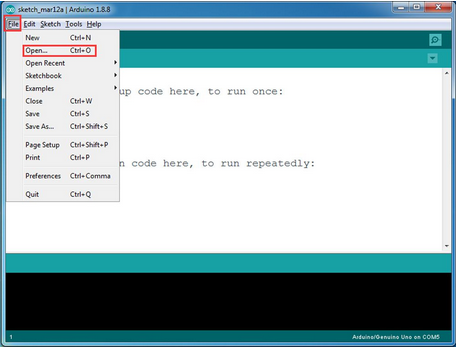
\includegraphics[width=0.7\linewidth]{Images/s2}
		\label{fig:s2}
	\end{figure}
	
	
	\item Choose the corresponding board/port for your project, and upload the sketch to the board.
	
	\begin{figure}[H]
		\centering
		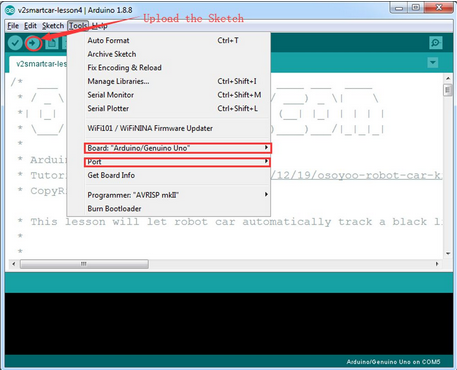
\includegraphics[width=0.7\linewidth]{Images/s3}
		\label{fig:s3}
	\end{figure}
	
	\item Adjust the sensitivity of tracking sensor modules. Turn on and hold the car and adjust the potentiometer on the tracking sensor with the Philips screwdriver. The signal LED light turns on when the sensor is above a black surface, and it turns off when the sensor is above the white surface.
	
\end{enumerate}
	
\textbf{NOTE}: The code provided is meant to work on a white surface with black tape. The competition will be held on a black surface with white tape. Also, while 5 sensors are provided in the kit, only 3 (left, right, middle) are used in the sample code. It is up to your group to determine how many of the sensors you wish to use. Use your creativity to adapt the code to this competition! 

\section{Extra Credit}

\paragraph{}For competition 1, the team will receive extra credit if they are able to stop the robot using the remote control once it has passed the finish line. Here is a guide to add the IR sensor to your robot.

\subsection{Hardware Installation}

\paragraph{}Please follow the instructions as listed to complete the build by the end of the Lab section. The instructions provided below are adapted from the OSOYOO provided instructions for your ease of use. If you wish to have additional support in the build process, navigate to the following link for a video tutorial. 

\href{https://osoyoo.com/2020/05/12/osoyoo-v2-1-robot-car-kit-lesson-2-ir-remote-control-robot-car/}{Video Tutorial Link}

\begin{enumerate}
	\item Add the IR receiver module onto the car. Install the IR receiver module with 2pcs M2.5*10 plastic screws, M2.5 plastic pillars and M2.5 plastic nuts at the front of the upper chassis.
	
	\begin{figure}[H]
		\centering
		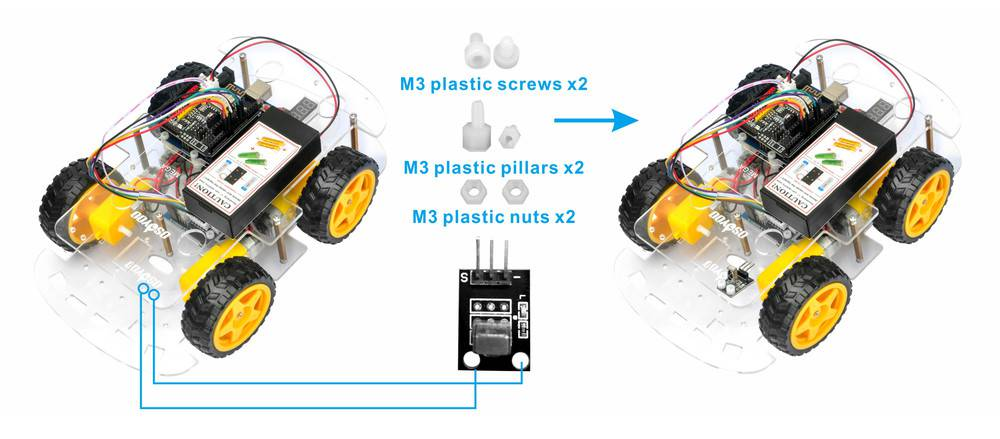
\includegraphics[width=0.7\linewidth]{Images/e1}
		\label{fig:e1}
	\end{figure}
	
	\item Connect the S pin in the IR receiver to the D10 pin in the UNO board, GND to GND, VCC to 5V, as the following photo (Remember : DO NOT remove any existing wires installed in Lesson 1 ).
	
	\begin{figure}[H]
		\centering
		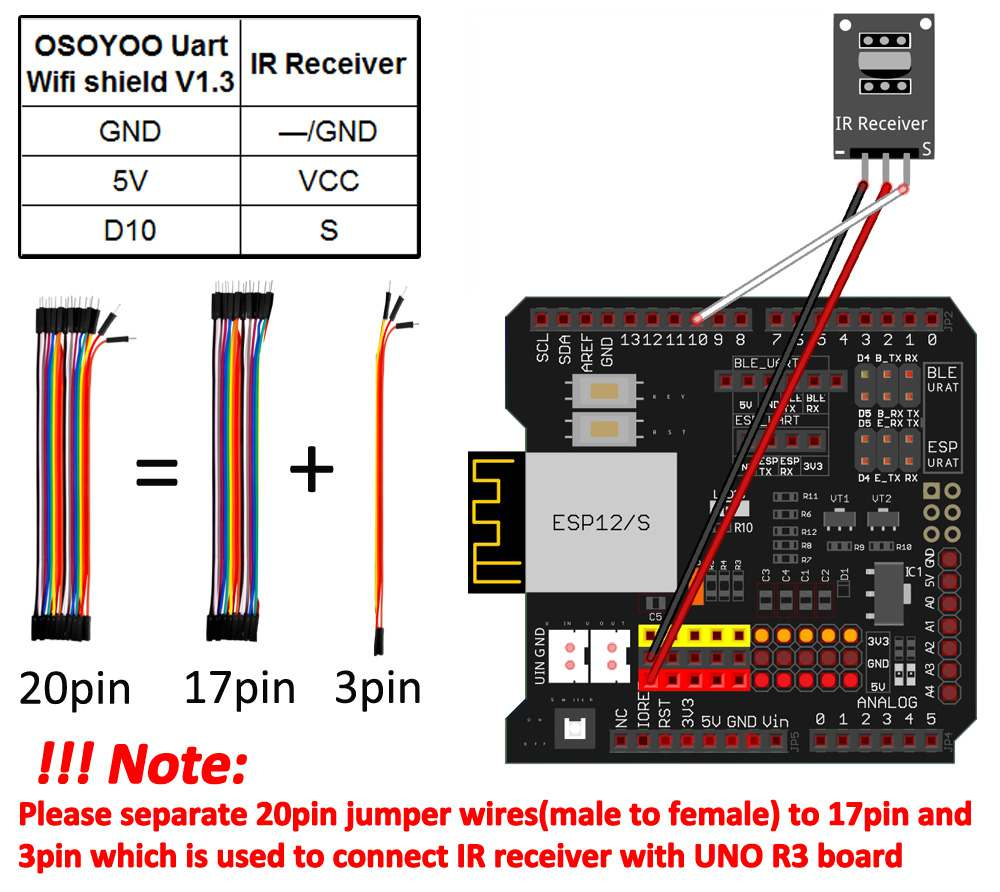
\includegraphics[width=0.5\linewidth]{Images/e2}
		\label{fig:e2}
	\end{figure}

\end{enumerate}


\subsection{Software Installation}
\begin{enumerate}
	\item Install IRremote library into Arduino IDE (If you have already installed IRremote library, please skip this step). Download IRremote library from \href{https://osoyoo.com/wp-content/uploads/samplecode/IRremote.zip}{this link}, then import the library into Arduino IDE(Open Arduino IDE $\rightarrow$ click Sketch $\rightarrow$ Include Library $\rightarrow$ Add .Zip Library)
	
	\begin{figure}[H]
		\centering
		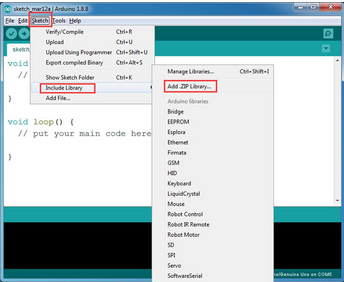
\includegraphics[width=0.7\linewidth]{Images/eSoftware1}
		\label{fig:esoftware1}
	\end{figure}
	
	
	\item Download Lesson 2 IRremote smart car sample code from \href{https://osoyoo.com/driver/v2smartcar-lesson2.zip}{this link} and unzip the download zip file smartcar-lesson2.zip, you will see a folder called smartcar-lesson2.
	
	\item Connect UNO R3 board to PC with USB cable, Open Arduino IDE $\rightarrow$ click file $\rightarrow$ click Open $\rightarrow$ choose code “smartcar-lesson2.ino” in smartcar-lesson2 folder, load the code into arduino.
	
	\begin{figure}[H]
		\centering
		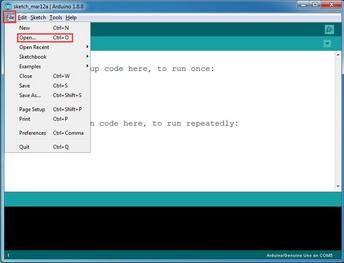
\includegraphics[width=0.7\linewidth]{Images/eSoftware3}
		\caption{}
		\label{fig:esoftware3}
	\end{figure}
	
	
	\item Choose corresponding board and port for your project,upload the sketch to the board.
\end{enumerate}


\subsection{Testing}

\paragraph{} Press IR controller keys to control the car movements as per following instruction table.

\begin{figure}[H]
	\centering
	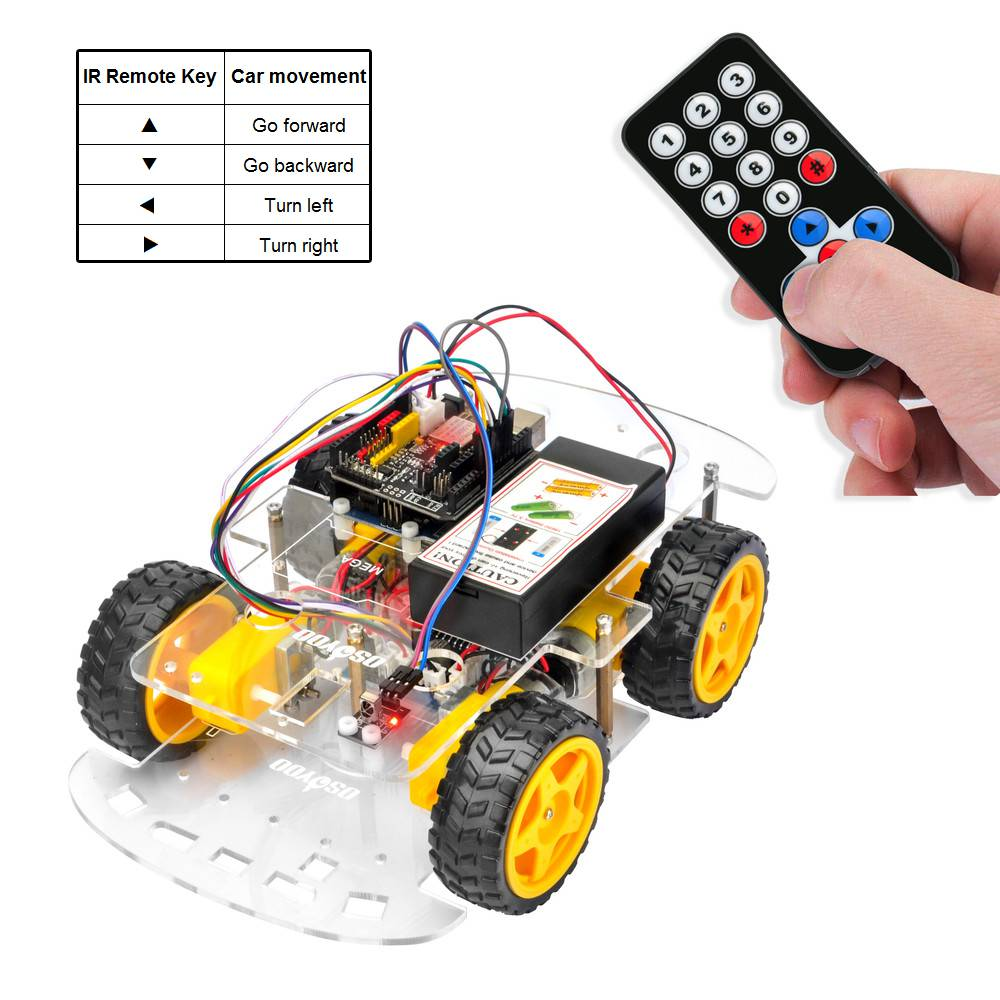
\includegraphics[width=0.5\linewidth]{Images/testing1}
	\label{fig:testing1}
\end{figure}

\subsection{Troubleshooting}

\paragraph{} In the unlikely event that the IR remote controller does not seem to work, refer to the troubleshooting section on \href{https://osoyoo.com/2020/05/12/osoyoo-v2-1-robot-car-kit-lesson-2-ir-remote-control-robot-car/}{this page}

\paragraph{}Now you should have the IR sensor and the tracking sensor module connected. Develop a code that makes the robot follow the white line and that can be stopped using the IR controller.
\end{document}
